\subsection{Discussion} \label{Sec:discussion}
\begin{figure}[!t]
  \centering
  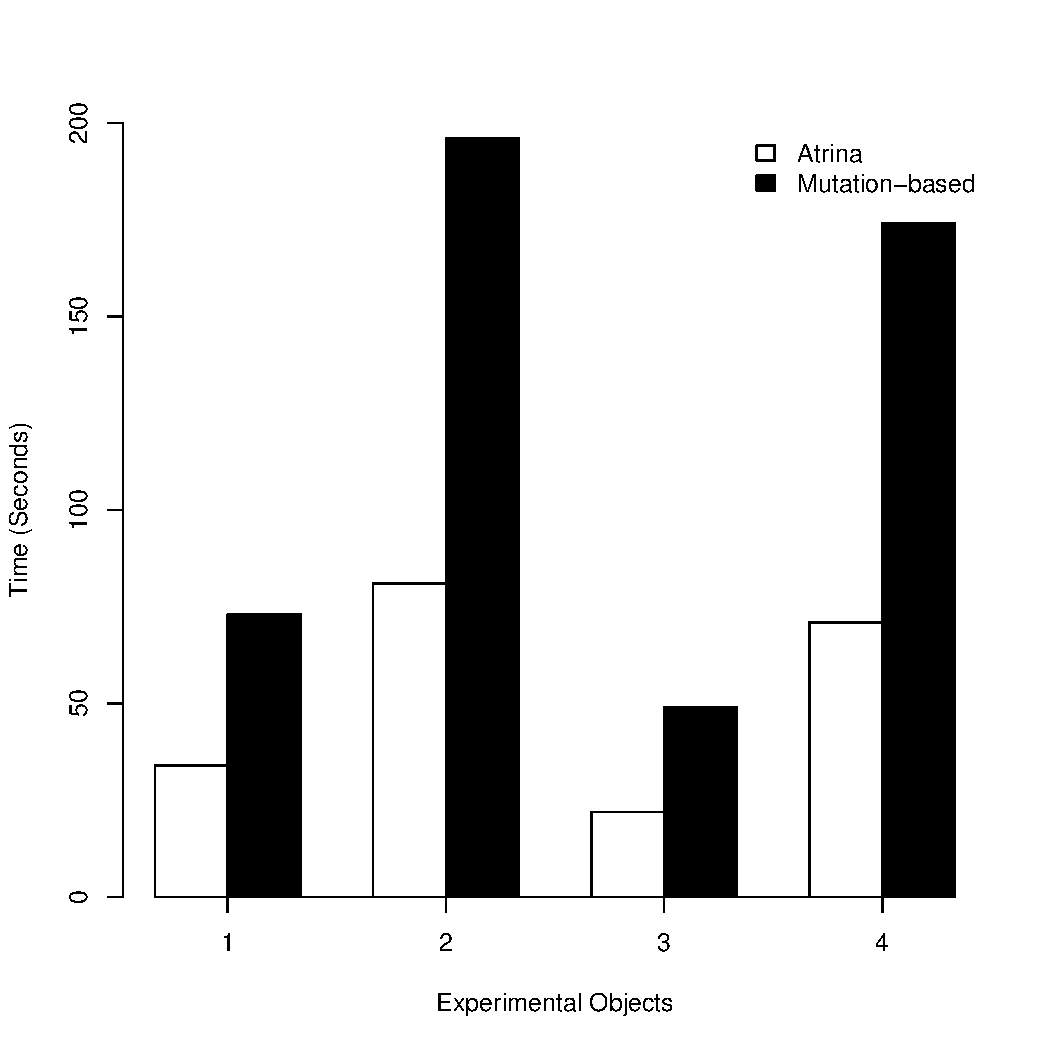
\includegraphics[width=0.7\hsize]{r-scripts/performance}
  \vspace{-0.18in}   
  \mycaption{Time overhead for each approach.}
  \vspace{-0.3in} 
  \label{Fig:performance}   
\end{figure}
\headbf{Time Efficiency} While the results demonstrate that \tool is more effective than mutation-based approach in terms of fault detection, we further investigate efficiency of our approach in terms of time overhead. 
We compute overhead of \tool as the summation of time required for (1) instrumenting the application, and (2) analyzing the collected trace to compute \javascript slices. To calculate time overhead of the mutation-based approach, we consider the total time required for running the test suite multiple times (once per mutation), generating mutants, as well as the time needed to compare the original and the mutated version of the application to generate assertions. \figref{performance} shows the results of time overhead computed for each approach.    
Our results show that the time overhead for \tool is 52 seconds on average, while the overhead computed for mutation-based technique is 123 seconds on average. As shown in the figure, for the EnterpriseStore application (ID 2), which is the largest application we considered (57K LOC), time efficiency is increased by 58\% using \tool. This indicates that our approach significantly outperforms mutation-based assertion generation as far as time efficiency is concerned. 
%Moreover, this reiterates the known performance shortcomings of approaches that rely on mutant generation.
\headbf{Fault Masking} As we mentioned in \secref{explicitAssertions}, the concrete value of an entity in the computed backward slice can potentially be used as the expected value of the entity in explicit assertions to test the current version of the application.
The actual values of the related entities in the backward slice are correct unless there exists a masked fault which is concealed in the chain of computations and thus does not propagate to the checked state of the DOM element. However, we conjecture that fault masking rarely happens in \javascript web applications as it is more prevalent in programs with many small expressions whose results are stored in several intermediate values. We also observed no fault masking occurrence during the evaluation of \tool on four \javascript applications used in this study.
\headbf{Limitations} The effectiveness of the generated assertions by \tool in terms of fault finding capability depends on the quality of human-written DOM-based test cases. If the DOM assertions contained in the DOM-based test suite check useless information, the explicit assertions obtained by our tool point to entities that may not be important from the tester's point of view. This can also negatively affect the fault finding capability of implicit assertions as they are indirectly inferred from the DOM-based assertions. Moreover, if the human-written test suite does not execute application's state with effective DOM elements, our tool is not able to infer effective candidate assertions.   